\chapter{Introducción al régimen transitorio}
	
\section{Introducción al régimen transitorio}
	
Cuando se produce un cambio en las condiciones de funcionamiento de un
circuito eléctrico (activación o apagado de fuentes, cambio en las
cargas, cambio en el circuito, apertura o cierre de interruptores...),
existe un periodo de transición en el que corrientes y tensiones en
las diferentes partes del circuito varían hasta alcanzar nuevos
valores. Este período se denomina \textbf{régimen transitorio}. Cuando
el circuito se estabiliza (tensiones y corrientes son constantes --en
continua-- o periódicas --en alterna--), se dice que está en
\textbf{régimen permanente}. Aplicando las leyes de Kirchhoff, se
llegará a escribir las ecuaciones del circuito, que quedarán
expresadas por una o varias ecuaciones diferenciales. Debe recordarse
la expresión de definición de tensión y corriente para bobinas y
condensadores, respectivamente:
\begin{align*}
  u_L(t) &= L \cdot \diff{i_L(t)}{t}
           \leftrightarrow
           i_L(t) = \frac{1}{L} \int^t_{-\infty}u_L(t') \mathrm{d}t'\\
  i_C(t) &= C \cdot \diff{u_C(t)}{t}
           \leftrightarrow
           u_C(t) = \frac{1}{C} \int^t_{-\infty}i_C(t') \mathrm{d}t'
\end{align*}
Por ejemplo, la ecuación de un circuito RLC en serie es de la forma:
\begin{equation*}
  a \cdot \diff[2]{f(t)}{t} + b \cdot \diff{f(t)}{t} + c \cdot f(t) = g(t)
\end{equation*}
cuya solución para $t > 0$ (\textbf{respuesta completa} del circuito
lineal al transitorio) tiene dos componentes:
\begin{equation*}
  f(t) = f_n(t) + f_\infty(t)
\end{equation*}
$f_n(t)$ se obtiene resolviendo la \textbf{ecuación homogénea} de la
ecuación diferencial (\textbf{respuesta natural}, equivalente a la
solución general $y_g$ de la ecuación diferencial), y representa la
respuesta de un circuito cuando se anulan los generadores existentes
en el mismo y donde se consideran únicamente como ``fuentes'' las
debidas a las energías almacenadas en los elementos reactivos de la
red (bobinas y condensadores); además, contiene las constantes de
integración de la ecuación diferencial correspondiente, calculadas a
partir de las condiciones iniciales del circuito. Estas condiciones
iniciales (en $t=0$) se determinan a partir de las condiciones de
continuidad en los elementos que almacenan energía (bobinas y
condensadores), sustituyendo dichos elementos por sus circuitos
equivalentes en el instante de tiempo dado. El otro término que se
incluye en la solución, $f_\infty(t)$, depende del tipo de excitación
del circuito y corresponde a la \textbf{solución forzada}
(particular), puesto que depende de la forma particular de la/s
fuente/s de excitación, y se corresponde con la solución en régimen
permanente (que ha sido estudiada en el resto de la
asignatura). Basándose en el orden $n$ que tenga la expresión
diferencial a resolver, los circuitos serán de orden uno, dos o
superior. En este caso, se va a trabajar únicamente circuitos de orden
uno y dos, que corresponden con circuitos eléctricos simples en serie
o paralelo:
\begin{itemize}
\item \textbf{Circuitos de primer orden.} Son aquellos que incluyen
  únicamente una bobina o un condensador
\item \textbf{Circuitos de segundo orden.} Son aquellos que incluyen
  dos bobinas o dos condensadores, o bien una bobina y un condensador
\end{itemize}

% \begin{remark}
%   Es importante recordar aquí el operador $D$, ya presentado en la
%   Sección~\ref{sec:operador_D}, puesto que permite escribir las
%   ecuaciones integro-diferenciales de los circuitos de una forma más
%   compacta (en el caso de los elementos pasivos, da lugar al
%   concepto de impedancia operacional):
%   \begin{align*}
% 	    Z_R(D)&=\dfrac{u_R(t)}{i(t)}=R\\
% 	    Z_L(D)&=\dfrac{u_L(t)}{i(t)}=LD\\
% 	    Z_C(D)&=\dfrac{u_C(t)}{i(t)}=\dfrac{1}{CD}
% 	\end{align*}
% \end{remark}
		
\subsection{Impedancia operacional: el operador $D$
}\label{sec:operador_D}
Las relaciones entre tensión y corriente de resistencias, bobinas y
condensadores, pueden escribirse mediante el empleo del operador
$D$. Este operador es equivalente a:
\begin{equation*}
  D\equiv \dfrac{d(...)}{dt} \rightarrow \dfrac{1}{D}=D^{-1}\equiv \int (...) dt
\end{equation*}
Estos operadores matemáticos permiten definir la \textbf{impedancia
  operacional} $Z(D)$, que puede representar un único elemento pasivo
simple ($R$, $L$ o $C$) o una combinación de ellos. Con este concepto,
la ley de Ohm queda como (\textbf{ley de Ohm generalizada}):
\begin{equation*}
  u(t)=Z(D)\cdot i(t)
\end{equation*}
siendo así la impedancia un cociente entre tensión y corriente, por lo
que tiene unidad de Ohmios [$\Omega$].  Con esto, las impedancias
operaciones de los elementos pasivos son:
\begin{align*}
  Z_R(D)&=\dfrac{u_R(t)}{i(t)}=R\\
  Z_L(D)&=\dfrac{u_L(t)}{i(t)}=LD\\
  Z_C(D)&=\dfrac{u_C(t)}{i(t)}=\dfrac{1}{CD}
\end{align*}
	
Análogamente, puede definirse la \textbf{admitancia operacional}
$Y(D)$:
\begin{equation*}
  Y(D)=\dfrac{1}{Z(D)}
\end{equation*}
con la que se cumple que:
\begin{equation*}
  i(t)=Y(D)\cdot u(t)
\end{equation*}
La admitancia es, entonces, un cociente entre corriente y tensión, con
unidad de Siemens [S]. Las admitancias operacionales de los elementos
pasivos son:
\begin{align*}
  Y_R(D)&=\dfrac{i(t)}{u_R(t)}=\dfrac{1}{R}=G\\
  Y_L(D)&=\dfrac{i(t)}{u_L(t)}=\dfrac{1}{LD}\\
  Y_C(D)&=\dfrac{i(t)}{u_C(t)}=CD
\end{align*} 

\section{Condiciones iniciales}\label{sec:condiciones_iniciales}
	
El instante del cambio en el circuito se representa habitualmente con
$t = 0$, siendo:
\begin{itemize}
\item $t = 0^-$ el tiempo inmediatamente anterior al cambio
\item $t = 0^+$ el tiempo inmediatamente posterior al cambio
\end{itemize}
Las condiciones iniciales de una red dependen de las energías
almacenadas en los elementos reactivos en $t=0^-$ y la estructura
topológica de la misma en $t=0^+$. Lo que haya pasado antes se
manifestará en los valores que tengan las tensiones en los
condensadores y las corrientes en las bobinas. Los detalles de este
proceso no tienen importancia y lo único que interesa es conocer los
valores en $t=0^-$. Una vez realizada la conmutación, en $t=0^+$,
pueden aparecer nuevas tensiones y corrientes en la red como resultado
de los valores iniciales anteriores y debido a las fuentes que ahora
se introducen o desaparecen. La evaluación de las tensiones y
corrientes en $t=0^+$ permitirá determinar las constantes de
integración que aparecen en la respuesta completa de la red para
$t>0$. Se presenta a continuación el comportamiento de los elementos
pasivos simples en el momento de la conmutación.
	
\subsection{Resistencia}
En una resistencia, la relación entre la tensión y la corriente viene
expresada por la ley de Ohm:
\begin{equation*}
  u_R(t)=R\cdot i_R(t)
\end{equation*}
Puesto que no hay acumulación de energía, y según la ecuación
anterior, la corriente en una resistencia sigue los cambios (la forma)
que imponga la tensión, si esta cambia instantáneamente, la corriente
también cambiará de un modo instantáneo, con una magnitud $1/R$ de la
tensión, sin producir dañado.
	
\subsection{Bobina}
Por la relación entre tensión y corriente en una bobina, se deduce que
la corriente \textbf{no puede variar bruscamente}, ya que la tensión
debería hacerse infinita, lo cual no tiene sentido físico:
\begin{equation*}
  u_L(t) = L \cdot \diff{i_L(t)}{t}
  \leftrightarrow
  i_L(t) = \frac{1}{L} \int^t_{-\infty}u_L(t') \mathrm{d}t'= \frac{1}{L} \int^{0^-}_{-\infty}u_L(t')\mathrm{d}t' + \frac{1}{L} \int^{t}_{0^-}u_L(t')\mathrm{d}t'
\end{equation*}
El primer sumando representa el valor de la corriente en $t=0^-$; si
la conmutación se realiza en $t=0$ y se desea calcular la corriente en
el instante $t=0^+$, resulta:
\begin{equation*}
  i_L(0^+)=i_L(0^-)+ \dfrac{1}{L}\cancelto{0}{\int_{0^-}^{0^+} u_L(t)\, dt}
\end{equation*}
siempre y cuando $u_L(t)$ sea finita. Por tanto, se deduce que:
\begin{equation}\label{eq:continuidad-bobina}
  \boxed{i_L(0^+)=i_L(0^-)}
\end{equation}
que representa la continuidad física de la corriente en la bobina en
el momento de la conmutación. De la
ecuación~\eqref{eq:continuidad-bobina} se deduce que, para el cálculo
de los valores iniciales en un circuito, \textbf{una bobina
  inicialmente cargada (IC) se puede sustituir por una fuente ideal de
  corriente de valor $i_g=i_L(0^+)=i_L(0^-)$ en paralelo con una
  bobina descargada (ID)}, como en la
Figura~\ref{fig:condiciones_iniciales_L}. Si la bobina está descargada
($i_L(0^-)=0$), se comporta inicialmente como un \textbf{circuito
  abierto}, independientemente de la tensión en sus terminales.
\begin{figure}[H]
  \centering 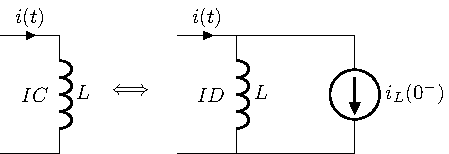
\includegraphics{../figs/condiciones_iniciales_L.pdf}
  \caption{Circuito equivalente de una bobina inicialmente cargada}
  \label{fig:condiciones_iniciales_L}
\end{figure}
	
% Otra conclusión es que pueden deducirse de es el comportamiento de
% una bobina cuando las excitaciones del circuito (generadores) son de
% corriente continua. En este caso, cuando se ha alcanzado el régimen
% permanente ($t=\infty$), la corriente en la bobina tendrá un valor
% constante independiente del tiempo, por lo que, según, la derivada
% será igual a 0, lo que significa que, \textbf{con corriente
% continua, en régimen permanente, una bobina se comporta como un
% cortocircuito}.
	
\subsection{Condensador}
Por la relación entre tensión y corriente en un condensador, se deduce
que la tensión \textbf{no puede variar bruscamente}, ya que la
corriente debería hacerse infinita, lo cual no tiene sentido físico:
\begin{equation*}
  i_C(t) = C \cdot \diff{u_C(t)}{t}
  \leftrightarrow
  u_C(t) = \frac{1}{C} \int^t_{-\infty}i_C(t') \mathrm{d}t'= \frac{1}{C} \int^{0^-}_{-\infty}i_C(t')\mathrm{d}t' + \frac{1}{C} \int^{t}_{0^-}i_C(t')\mathrm{d}t'
\end{equation*}
El primer sumando representa el valor de la tensión en $t=0^-$; si la
conmutación se realiza en $t=0$ y se desea calcular la corriente en el
instante $t=0^+$, resulta:
\begin{equation*}
  u_C(0^+)=u_C(0^-)+ \dfrac{1}{C}\cancelto{0}{\int_{0^-}^{0^+} i_C(t)\, dt}
\end{equation*}
siempre y cuando $i_C(t)$ sea finita. Por tanto, se deduce que:
\begin{equation}\label{eq:continuidad-condensador}
  \boxed{u_C(0^+)=u_C(0^-)}
\end{equation}
que representa la continuidad física de la tensión en el condensador
en el momento de la conmutación. De la
ecuación~\eqref{eq:continuidad-condensador} se deduce que, para el
cálculo de los valores iniciales en un circuito, \textbf{un
  condensador inicialmente cargado (IC) se puede sustituir por una
  fuente ideal de tensión de valor $u_g=u_C(0^+)=u_C(0^-)$ en serie
  con un condensador descargado (ID)}, como en la
Figura~\ref{fig:condiciones_iniciales_C}. Si el condensador está
descargado ($u_C(0^-)=0$), se comporta inicialmente como un
\textbf{cortocircuito}, independientemente de la corriente que circule
por el mismo.
\begin{figure}[H]
  \centering 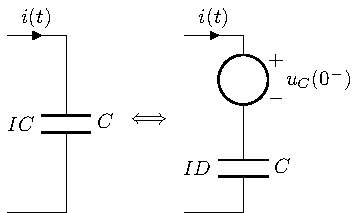
\includegraphics{../figs/condiciones_iniciales_C.pdf}
  \caption{Circuito equivalente de un condensador inicialmente
    cargado}
  \label{fig:condiciones_iniciales_C}
\end{figure}
	
	
\subsection{Procedimiento general para obtener las condiciones
  iniciales} \label{sec:proc_general_ci} Cuando se desean determinar
las condiciones iniciales de una red, deben seguirse los siguientes
pasos:
\begin{enumerate}
\item Sustituir los generadores de tensión del circuito
  $\epsilon_g(t)$ por fuentes de tensión continua de valor
  $\epsilon_g(0^+)$.
\item Sustituir todos los generadores de corriente del circuito
  $i_g(t)$ por fuentes de corriente continua de valor $i_g(0^+)$.
\item Sustituir todas las bobinas cargadas por su circuito equivalente
  con condiciones iniciales $i_L(0^-)=i_L(0^+)$. Si la corriente
  inicial en la bobina es 0 ($i_L(0^-)=0$), se sustituye por un
  circuito abierto.
\item Sustituir todos los condensadores cargados por su circuito
  equivalente con condiciones iniciales $u_C(0^+)=u_C(0^-)$. Si la
  tensión inicial en un condensador es 0 ($u_C(0^-)=0$), se sustituye
  por un cortocircuito.
\item En la red resistiva resultante, calcular las corrientes y
  tensiones iniciales necesarias para el estudio subsiguiente de la
  red.
\end{enumerate}
	
\begin{example}\label{ex.condiciones_iniciales}
  \textbf{En la red de la Figura~\ref{fig:ej_condiciones_iniciales},
    la corriente del generador de intensidad es
    $i_g(t) = 10\,\mathrm{e}^{-2t}$ A. El interruptor se abre en
    $t = 0$, siendo los valores iniciales $i_L(0^-) = 0$ A;
    $u_C(0^-) = -5$ V. Se pide calcular $i_R(0^+)$, $i_C(0^+)$ y
    $u_L(0^+)$.}
  \begin{figure}[H]
    \centering 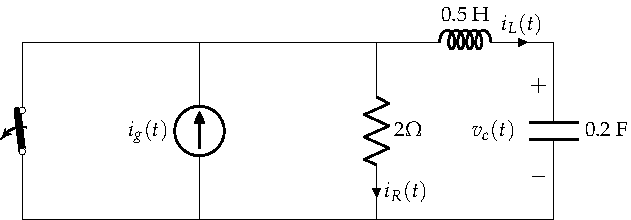
\includegraphics{../figs/ej_condiciones_iniciales.pdf}
    \caption{Ejemplo~\ref{ex.condiciones_iniciales}}
    \label{fig:ej_condiciones_iniciales}
  \end{figure}

  Siguiendo el procedimiento general de la
  Sección~\ref{sec:proc_general_ci}:
  \begin{enumerate}
  \item Sustituir los generadores de tensión del circuito
    $\epsilon_g(t)$ por fuentes de tensión continua de valor
    $\epsilon_g(0^+) \rightarrow$ no existen generadores de tensión
  \item Sustituir todos los generadores de corriente del circuito
    $i_g(t)$ por fuentes de corriente continua de valor
    $i_g(0^+)\rightarrow$ se sustituye la fuente de corriente por una
    de valor $i_g(0^+)=10\,\mathrm{e}^{-2\cdot 0}=10$ A
  \item Sustituir todas las bobinas cargadas por su circuito
    equivalente con condiciones iniciales $i_L(0^-)=i_L(0^+)$. Si la
    corriente inicial en la bobina es 0 ($i_L(0^-)=0$), se sustituye
    por un circuito abierto $\rightarrow$ dado que $i_L(0^-)=0$, se
    sustituye la bobina por un circuito abierto
  \item Sustituir todos los condensadores cargados por su circuito
    equivalente con condiciones iniciales $u_C(0^+)=u_C(0^-)$. Si la
    tensión inicial en un condensador es 0 ($u_C(0^-)=0$), se
    sustituye por un cortocircuito $\rightarrow$ se sustituye el
    condensador inicialmente cargado por uno incialmente descargado en
    serie con una fuente de tensión de valor $-5$ V
  \end{enumerate}
  Con estas consideraciones, la red quedaría como se muestra en la
  Figura~\ref{fig:ej_cond_iniciales_0+}. Debe destacarse que este
  circuito es \textbf{únicamente válido para este instante de tiempo},
  $t=0^+$. Al tratarse, además, de un circuito de corriente continua
  en este instante, el condensador descargado quedaría como un
  cortocircuito.
  \begin{figure}[H]
    \centering 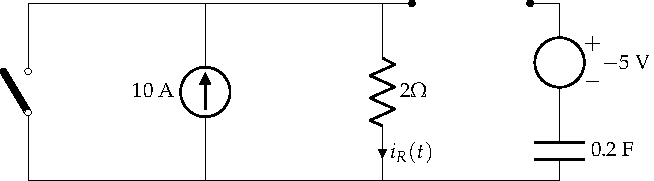
\includegraphics{../figs/ej_cond_iniciales_0+.pdf}
    \caption{Circuito equivalente para condiciones iniciales}
    \label{fig:ej_cond_iniciales_0+}
  \end{figure}
	
  Con estas consideraciones, y aplicando la ley de Ohm y las leyes de
  Kirchhoff, se obtiene que:
  \begin{align*}
    i_R(0^+)&=10\,A\\
    i_C(0^+)&=0\,A\\
    u_L(0^+)&10\cdot 2 - (-5)=25\,V
  \end{align*}
	
\end{example}

	
\section{Circuitos de primer orden}\label{sec:primer_orden}
	
Se estudian los circuitos cuyo modelo matemático es una ecuación
diferencial lineal de primer orden. Físicamente, estos circuitos están
constituidos por un número cualquiera de resistencias y fuentes
independientes, pero con \textbf{un único elemento reactivo} (o varios
del mismo tipo que puedan ser sustituidos por uno equivalente por
estar asociados en serie o paralelo). La ecuación homogénea del
circuito ($g(t)=0$) es de la forma:
\begin{equation*}
  a_1\,y'(t)+a_0\,y(t)=0\Rightarrow y'(t)+\dfrac{a_0}{a_1}\,y(t)=0
\end{equation*}
El método más inmediato para analizar estos circuitos en régimen
transitorio consiste en escribir la ecuación diferencial de la
variable en estudio y resolverla a partir de las condiciones iniciales
conocidas. %Así, el polinomio característico asociado a la expresión anterior es:
% \begin{equation*}
% 	    \lambda + \dfrac{a_0}{a_1}=0\Rightarrow \lambda = -\dfrac{a_0}{a_1}=-\dfrac{1}{\tau} 
% 	\end{equation*}
% 	donde $\tau=\frac{a_1}{a_0}$ es conocido como la
%  \textbf{constante de tiempo} del
%  circuito. %, que representa el tiempo que tardaría la función en alcanzar su valor final, si siguiera creciendo al mismo ritmo que en el origen.
La solución de la ecuación homogénea ({respuesta natural}) es:
\begin{equation}\label{eq:respuesta_natural_1}
  \boxed{y_n(t)=K\,\mathrm{e}^{-\frac{a_0\,t}{a_1}}}
\end{equation}
siendo $K$ una constante de integración cuyo valor se obtiene a partir
de las condiciones iniciales una vez se obtiene la solución
particular, $y_{\infty}(t)$. Puesto que se tiene que:
\begin{equation*}
  y(t)=y_n(t)+y_\infty(t)=K\,\mathrm{e}^{-\frac{a_0\,t}{a_1}}+y_\infty(t)
\end{equation*}
en el instante de tiempo $t=0^+$:
\begin{equation}\label{eq:ecuacion_1orden}
  y(0^+)=K+y_\infty(0^+)\Rightarrow K=y(0^+)-y_\infty(0^+)\Rightarrow \boxed{y(t)=\underbrace{\left[y(0^+)-y_\infty(0^+) \right]}_{K}\,\mathrm{e}^{-\frac{a_0\,t}{a_1}}+y_\infty(t)}
\end{equation}
% Según el elemento reactivo que se tenga, el valor de $\tau$ es:
% \begin{itemize}
% \item \textbf{Bobinas:}
%   \begin{equation}\label{eq:tau_L}
% 	        \boxed{\tau=\dfrac{L}{R_{th}}}
% 	    \end{equation}
%    \item \textbf{Condensadores:}
% 	    \begin{equation}\label{eq:tau_C}
% 	        \boxed{\tau=C\cdot R_{th}}
% 	    \end{equation}
%    \end{itemize}
%    donde la $R_{th}$ es la resistencia vista desde los bornes del
%    condensador o de la bobina, cuando se anulan todas las fuentes
%    independientes (es decir, la resistencia de Thévenin).
	
\subsection{Circuito RC paralelo}
Sea el circuito RC mostrado en la Figura~\ref{fig:transitorio_RC},
donde se cumple que en $t = 0$ se cierra el interruptor, alimentando
al condensador, que está descargado inicialmente.
\begin{figure}[H]
  \centering 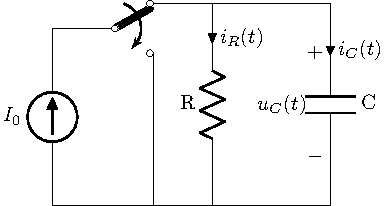
\includegraphics{../figs/transitorio_circuitoRC.pdf}
  \caption{Análisis transitorio de un circuito RC paralelo}
  \label{fig:transitorio_RC}
\end{figure}
	
Una vez se cierra el interruptor, por la 1LK, se cumple que:
\begin{equation*}
  i_R(t) + i_C(t) = I_0
\end{equation*}
donde, por definición:
\begin{equation*}
  i_R(t)=\dfrac{u_C(t)}{R}\qquad\qquad i_C(t)=C\,\diff{u_C(t)}{t}=C\,u_C'(t)
\end{equation*}
Por tanto, se obtiene la ecuación de primer orden que caracteriza a
este tipo de circuitos:
\begin{equation}\label{eq:1orden_C}
  \dfrac{u_C(t)}{R}+C\, u_C'(t)=\dfrac{u_C(t)}{R\,C}+u_C'(t)=\dfrac{I_0}{C}\Rightarrow \boxed{\dfrac{I_0}{C}=u_C'(t)+\dfrac{1}{R\, C}\,u_C(t)}
\end{equation}
	
La solución homogénea (\textbf{respuesta natural}) de esta ecuación,
siguiendo la expresión~\eqref{eq:respuesta_natural_1} es:
\begin{equation}
  \boxed{u_{C,n}(t)=K\,\mathrm{e}^{-\frac{t}{R\,C}}}
\end{equation}
Para determinar la solución particular (\textbf{respuesta forzada}),
se analiza el circuito con la fuente de alimentación. Al tratarse de
corriente continua, el condensador se comporta como un circuito
abierto (ver Sección~\ref{sec:condensador}), por lo que:
\begin{equation}
  \boxed{u_{C,\infty}(t)=R\cdot I_0}
\end{equation}
Por tanto, la solución completa de la ecuación diferencial es, a falta
de determinar $K$:
\begin{equation*}{u_C(t)=K\,\mathrm{e}^{-\frac{t}{R\,C}}+R\cdot I_0}
\end{equation*}
Puesto que el condensador estaba inicialmente descargado,
$u_C(0^-)=0$, por continuidad, se tiene entonces que
$u_C(0^+)=u_C(0^-)=0$. Sustituyendo en la solución completa el valor
de $t$ por $t=0^+$, se obtiene que:
\begin{equation*}
  u_C(0^+)=0=K\,\cancelto{1}{\mathrm{e}^{-\frac{0^+}{R\,C}}}+R\cdot I_0\Rightarrow K=-R\cdot I_0
\end{equation*}
siendo la solución completa:
\begin{equation}\label{eq:uc-completa-1}
  u_C(t)=-R\cdot I_0\,\mathrm{e}^{-\frac{t}{R\,C}}+R\cdot I_0\Rightarrow \boxed{u_C(t) =R\cdot I_0\left(1- \mathrm{e}^{-\frac{t}{R\,C}}\right)}
\end{equation}
	
Si en la expresión~\eqref{eq:uc-completa-1} se hace $t=\infty$,
resulta:
\begin{equation*}
  u_C(\infty)=R\cdot I_0\left(1- \cancelto{0}{\mathrm{e}^{-\frac{\infty}{R\,C}}}\right)=R\cdot I_0
\end{equation*}
que es la tensión en \textbf{régimen permanente} en el
condensador. Por tanto, la respuesta de $u_C(t)$ dada por la
ecuación~\eqref{eq:uc-completa-1} puede considerarse como la suma de
la respuesta en régimen permanente más una respuesta transitoria que
se amortigua con el tiempo y cuya contribución a la respuesta total
será despreciable a partir de un cierto instante (cuando haya
desaparecido el régimen transitorio).
	
Al producto $R\,C$ se le denomina \textbf{constante de tiempo}, y
representa el tiempo que el condensador tardaría en cargarse de
continuar en todo momento la intensidad inicial $I_0$; también
equivale al tiempo necesario para que el condensador se cargue al 63\%
de su capacidad. Suele representarse por $\tau$ y se considera que,
para cinco veces el valor de la constante de tiempo ($5\tau$), el
condensador está completamente cargado:
\begin{equation}
  \boxed{\tau=R\,C}
\end{equation}

\subsection{Circuito RL serie}
	
Sea el circuito RL mostrado en la Figura~\ref{fig:transitorio_RL},
donde se cumple que en $t = 0$ se cierra el interruptor, alimentando a
la bobina, que está descargada inicialmente. Lógicamente, una vez
cerrado el interruptor, se cumple que $i_R(t)=i_L(t)$.
\begin{figure}[H]
  \centering 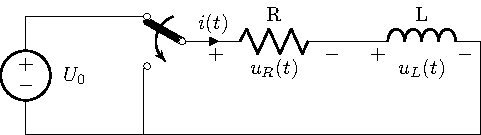
\includegraphics{../figs/transitorio_circuitoRL.pdf}
  \caption{Análisis transitorio de un circuito RL serie}
  \label{fig:transitorio_RL}
\end{figure}
	
Una vez se cierra el interruptor, por la 2LK, se cumple que:
\begin{equation*}
  u_R(t) + u_L(t) = U_0
\end{equation*}
donde, por definición:
\begin{equation*}
  u_R(t)=R\,i_L(t)\qquad\qquad u_L(t)=L\,\diff{i_L(t)}{t}=L\,i_L'(t)
\end{equation*}
Por tanto, se obtiene la ecuación de primer orden que caracteriza a
este tipo de circuitos:
\begin{equation}\label{eq:1orden_L}
  R\,i_L(t)+L\, i_L'(t)=\dfrac{R}{L}\,i_L+i_L'(t)=\dfrac{U_0}{L}\Rightarrow \boxed{\dfrac{U_0}{L}=i_L'(t)+\dfrac{R}{L}\,i_L(t)}
\end{equation}
	
La solución homogénea (\textbf{respuesta natural}) de esta ecuación,
siguiendo la expresión~\eqref{eq:respuesta_natural_1} es:
\begin{equation}
  \boxed{i_{L,n}(t)=K\,\mathrm{e}^{-\frac{R\,t}{L}}}
\end{equation}
Para determinar la solución particular (\textbf{respuesta forzada}),
se analiza el circuito con la fuente de alimentación. Al tratarse de
corriente continua, la bobina se comporta como un cortocircuito (ver
Sección~\ref{sec:bobina}), por lo que:
\begin{equation}
  \boxed{i_{L,\infty}(t)=\dfrac{U_0}{R}}
\end{equation}
Por tanto, la solución completa de la ecuación diferencial es, a falta
de determinar $K$, es:
\begin{equation}\label{eq:il-completa-1-sinK}
  i_L(t)=K\,\mathrm{e}^{-\frac{R\,t}{L}}+\dfrac{U_0}{R}
\end{equation}
Puesto que la bobina estaba inicialmente descargada, $i_L(0^-)=0$, por
continuidad, se tiene entonces que $i_L(0^+)=i_L(0^-)=0$. Sustituyendo
en la solución completa el valor de $t$ por $t=0^+$, se obtiene que:
\begin{equation*}
  i_L(0^+)=0=K\,\cancelto{1}{\mathrm{e}^{-\frac{R\,0^+}{L}}}+\dfrac{U_0}{R}\Rightarrow K=-\dfrac{U_0}{R}
\end{equation*}
siendo la solución completa:
\begin{equation}\label{eq:il-completa-1}
  i_L(t)=-\dfrac{U_0}{R}\,\mathrm{e}^{-\frac{R\,t}{L}}+\dfrac{U_0}{R} \Rightarrow \boxed{i_L(t) =\dfrac{U_0}{R}\left(1- \mathrm{e}^{-\frac{R\,t}{L}}\right)}
\end{equation}
Al cociente $\frac{R}{L}$ se le denomina \textbf{constante de tiempo}
$\tau$:
\begin{equation}
  \boxed{\tau=\dfrac{L}{R}}
\end{equation}
	
Si en la expresión~\eqref{eq:il-completa-1} se hace $t=\infty$,
resulta:
\begin{equation*}
  i_L(\infty) =\dfrac{U_0}{R}\left(1- \cancelto{0}{\mathrm{e}^{-\frac{R\,\infty}{L}}}\right)=\dfrac{U_0}{R}
\end{equation*}
que es la corriente en \textbf{régimen permanente} en la bobina. Por
tanto, la respuesta de $i_L(t)$ dada por la
ecuación~\eqref{eq:il-completa-1} puede considerarse como la suma de
la respuesta en régimen permanente más una respuesta transitoria que
se amortigua con el tiempo y cuya contribución a la respuesta total
será despreciable a partir de un cierto instante (cuando haya
desaparecido el régimen transitorio).
	
% La energía acumulada en la bobina en \(t < 0\) se disipa en la
% resistencia en \(t > 0\)

% \begin{equation*}
%   W_R = \int_0^\infty R i^2(t) \mathrm{d}t = \int_0^\infty R (I_0
%   e^{-\frac{t}{\tau}})^2 \mathrm{d}t = \frac{1}{2} L I_0^2 = W_L
% \end{equation*}
	
	
	
	
	
	
	
	
\subsection{Procedimiento general}
	
Supóngase un circuito eléctrico cualquiera como se muestra en la
Figura~\ref{fig:CE_primerorden} (C.E. es un circuito eléctrico que no
contiene ningún elemento almacenador de energía), en el que se
conectan entre los terminales $A-B$ un elemento almacenador de energía
(condensador o bobina). Si las variables a estudiar son la tensión en
el condensador $u_C(t)$ o la intensidad en la bobina $i_L(t)$,
respectivamente, dicho circuito eléctrico de primer orden se puede
convertir en los circuitos eléctricos mostrados en las Figuras
\ref{fig:transitorio_RC} y \ref{fig:transitorio_RL}, calculando el
equivalente de Norton o Thévenin de los dipolos, como se muestra en la
Figura~\ref{fig:thevenin_1orden}.
\begin{figure}[H]
  \centering
  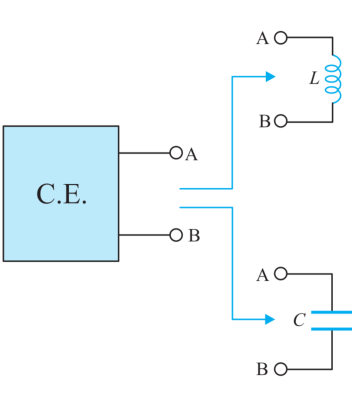
\includegraphics[width=0.3\linewidth]{../figs/CE_primerorden.pdf}
  \caption{Circuito eléctrico de primer
    orden} \label{fig:CE_primerorden}
\end{figure}
	
\begin{figure}[H]
  \centering \subfloat[Equivalente de
  Norton]{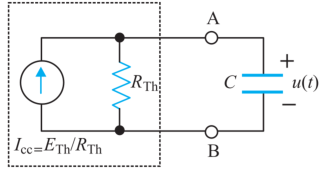
\includegraphics{../figs/thevenin_1orden_C.pdf}}\hfil
  \subfloat[Equivalente de
  Thévenin]{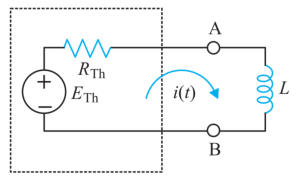
\includegraphics{../figs/thevenin_1orden_L.pdf}}
  \caption{Equivalentes de Norton y Thévenin para un circuito de
    primer orden}
  \label{fig:thevenin_1orden}
\end{figure}
Por tanto, las ecuaciones diferenciales de las variables $u_C(t)$ e
$i_L(t)$ son las dadas por las expresiones \eqref{eq:1orden_C} y
\eqref{eq:1orden_L}, sustituyendo $I_0$ por $i_{CC}(t)$, $U_0$ por
$\epsilon_{th}(t)$ y $R$ por $R_{th}$.
	
\begin{remark}
  $R_{th}$ es la resistencia vista desde los bornes del condensador o
  de la bobina, cuando se anulan todas las fuentes independientes.
\end{remark}
	
Dicho esto, el \textbf{proceso general} de cálculo de transitorios en
una red de primer orden sigue los siguientes pasos:
\begin{enumerate}
\item Dibujar el circuito para $t < 0$:
  \begin{itemize}
  \item Obtener el valor de $i_L(0^-)$ o $u_C(0^-)$
  \item Aplicar el principio de continuidad para determinar $i_L(0^+)$
    o $u_C(0^+)$ según lo indicado en la
    Sección~\ref{sec:condiciones_iniciales}
  \end{itemize}
\item Dibujar el circuito para \(t > 0\):
  \begin{itemize}
  \item Calcular el equivalente de Thévenin/Norton visto por el
    elemento acumulador de energía (en muchos casos, si el circuito es
    sencillo, basta con determinar $R_{th}$)
  \item Determinar el valor de la constante de tiempo del circuito:
    \begin{equation*}
      \tau = \dfrac{L}{R_{th}} \qquad\qquad \tau = R_{th}\,{C}
    \end{equation*}
  \item Calcular la respuesta en régimen permanente (solución
    particular, que corresponde a $t=\infty$), $i_\infty(t)$ o
    $u_\infty(t)$, teniendo en cuenta las siguientes consideraciones
    según el tipo de alimentación del circuito:
    \begin{enumerate}
    \item \textit{Corriente continua}: sustituir la bobina por un
      cortocircuito y el condensador por un circuito abierto
    \item \textit{Corriente alterna senoidal}: resolver el circuito
      por el método fasorial
    \item \textit{Otro tipo de forma de onda}: determinar la solución
      particular de la ecuación diferencial
    \end{enumerate}
  \end{itemize}
\item Escribir la solución completa para $t>0$:
  \begin{align*}
    i_L(t) &= \left(i_L(0^+) - i_\infty(0^+)\right) e^{-\frac{t}{\tau}} + i_\infty(t)\\
    u_C(t) &= \left(u_C(0^+) - u_\infty(0^+)\right) e^{-\frac{t}{\tau}} + u_\infty(t)\\
  \end{align*}
\end{enumerate}
	
\begin{example}\label{ex.primer_orden}
  \textbf{En el circuito de la Figura~\ref{fig:ej_transitorio_1orden},
    calcular la corriente $i(t)$ al cerrar el interruptor en $t = 0$
    s.}
  \begin{figure}[H]
    \centering 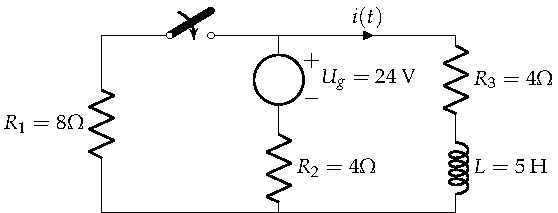
\includegraphics{../figs/ej_transitorio_1orden.pdf}
    \caption{Ejemplo~\ref{ex.primer_orden}}
    \label{fig:ej_transitorio_1orden}
  \end{figure}
	    
  \underline{Condiciones iniciales $t<0$}
	    
  Cuando $t=0^-$, el interruptor está abierto. Al tratarse de una
  fuente de alimentación de corriente continua, la bobina actúa como
  un cortocircuito. Por tanto:
  \begin{equation*}
    i(0^-)=\dfrac{U_g}{R_2+R_3}=\dfrac{24}{4+4}=3\,A
  \end{equation*}
	    
  Por continuidad:
  \begin{equation*}
    i_L(0^+)=i_L(0^-)=3\,A
  \end{equation*}
	    
  \underline{Circuito en $t>0$}
	    
  La resistencia de Thévenin vista desde la bobina, al no evistir
  fuentes dependientes, se puede determinar como la resistencia
  equivalente vista desde estos terminales al anular la fuente
  independiente:
  \begin{equation*}
    R_{th}=R_3+\dfrac{R_1\cdot R_2}{R_1+R_2}=4+\dfrac{8\cdot 4}{8+4}=\dfrac{20}{3}\Omega
  \end{equation*}
	    
  La constante de tiempo del circuito es:
  \begin{equation*}
    \tau=\dfrac{L}{R_{th}}=\dfrac{5}{\frac{20}{3}}=\dfrac{3}{4} \,s
  \end{equation*}
	    
  Para calcular la respuesta en régimen permanente, la bobina vuelve a
  sustituirse por un cortocircuito al tratarse de una excitación de
  corriente continua. Aplicando el método de nudos modificados:
  \begin{equation*}
    \dfrac{U}{R_1}+\dfrac{U-U_g}{R_2}+\dfrac{U}{R_3}=0\Rightarrow U=\dfrac{48}{5}\,V
  \end{equation*}
  por lo que:
  \begin{equation*}
    i_\infty(t)=\dfrac{U}{R_3}=\dfrac{\frac{48}{5}}{4}=\dfrac{12}{5}\,A
  \end{equation*}
  que, particularizada para $t=0^+$:
	    
  \begin{equation*}
    i_\infty(0^+)=\dfrac{12}{5}\,A
  \end{equation*}
	    
  \underline{Solución completa}
	    
  Por tanto, para $t>0$, la expresión de $i(t)$ (que se corresponde
  con $i_L(t)$ al ser la corriente que recorre la bobina) es:
  \begin{equation*}
    i_L(t)=\left(3-\dfrac{12}{5}\right)\,\mathrm{e}^{-\frac{4}{3}t}+\dfrac{12}{5}\,A=\dfrac{3}{5}\,\mathrm{e}^{-\frac{4}{3}t}+\dfrac{12}{5}\,A
  \end{equation*}
\end{example}
	
\begin{example}\label{ex.ejemplo_1orden_AC}
	
  \textbf{El conmutador del circuito de la
    Figura~\ref{fig:ej_transitorio_1orden_AC} pasa de la posición a 1
    a la 2 en $t = 0$ s. Calcular la tensión en bornes de la bobina
    $t > 0$ s.}
	
  \begin{figure}[H]
    \centering 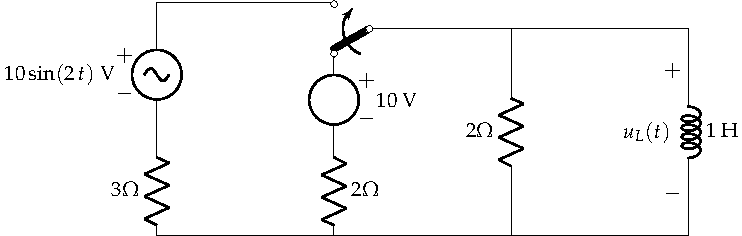
\includegraphics{../figs/ej_transitorio_1orden_AC.pdf}
    \caption{Ejemplo~\ref{ex.ejemplo_1orden_AC}}
    \label{fig:ej_transitorio_1orden_AC}
  \end{figure}
	    
  \underline{Condiciones iniciales $t<0$}
	
  Para $t<0$, el circuito es alimentado por una fuente de corriente
  continua, por lo que la bobina se comporta como un
  cortocircuito. Por tanto, toda la corriente circulará por dicha
  rama:
  \begin{align*}
    i_R&=0 \,A\\
    i_L&=\dfrac{10}{2}=5\,A
  \end{align*}
    
  Por continuidad, se tiene que:
  \begin{equation*}
    i_L(0^-)=i_L(0^+)=5\,A
  \end{equation*}
	
  \underline{Circuito en $t>0$}
	
  En $t=0$, el interruptor cambia de posición, y el circuito para a
  estar alimentado por una fuente de corriente alterna. La resistencia
  de Thévenin vista desde la bobina puede determinarse como la
  resistencia equivalente al no haber fuentes dependientes:
  \begin{equation*}
    R_{th}=\dfrac{2\cdot 3}{2+3}=1.2\,\Omega
  \end{equation*}
  y la constante de tiempo del circuito:
  \begin{equation*}
    \tau=\dfrac{L}{R_{th}}=\dfrac{1}{1.2}=\dfrac{5}{6}\,s
  \end{equation*}
	
  La fem del generador de Thévenin desde los terminales de la bobina:
  \begin{equation*}
    \overline{\epsilon_{th}}=2\cdot \underbrace{\dfrac{10\phase{0^\circ}}{2+3}}_{\overline{I}}=4\phase{0^\circ}\,V
  \end{equation*}
	
  Con el equivalente de Thévenin se calcula la corriente que circula
  por la bobina en régimen permanente:
  \begin{align*}
    \overline{I_L}&=\dfrac{\overline{\epsilon_{th}}}{R{th}+\overline{Z_L}}=\dfrac{4\phase{0^\circ}}{1.2+\mathrm{j}\,2\,1}=1.715\phase{-59.036^\circ} A\\
                  &i_\infty(t)=1.715\,\sin(2\,t-1.030)\,A
  \end{align*}
  que, particularizada para $t=0^+$:
  \begin{equation*}
    i_\infty(0^+)=1.715\,\sin(2\,0-1.030)=-1.47\,A
  \end{equation*}
	
  \underline{Solución completa}
	
  La solución completa para $i_L(t)$ es:
  \begin{equation*}
    i_L(t)=(5-(-1.47))\,\mathrm{e}^{-\frac{6\,t}{5}}+1.715\,\sin(2\,t-1.030)=6.47\,\mathrm{e}^{-\frac{6\,t}{5}}+1.715\,\sin(2\,t-1.030)\,A
  \end{equation*}
	
  Aplicando la ley de Ohm en la bobina:
  \begin{equation*}
    u_L(t)=Z_L\,i_L(t)=L\,D\,i_L=L\diff{i_L(t)}{t}
  \end{equation*}
  Haciendo la derivada de la corriente en la bobina respecto al
  tiempo:
  \begin{align*}
    \diff{i_L(t)}{t}&=-\dfrac{6}{5}\cdot 6.47\,\mathrm{e}^{-\frac{6\,t}{5}}+2\cdot 1.715\cos(2\,t-1.030)\\
                    &=-7.764\,\mathrm{e}^-{\frac{6\,t}{5}}+3.43\cos(2\,t-1.03)\,V
  \end{align*}
  Por tanto, la tensión de la bobina, dado que $L=1$ H:
  \begin{equation*}
    u_L(t)=-7.764\,\mathrm{e}^-{\frac{6\,t}{5}}+3.43\cos(2\,t-1.03)\,V
  \end{equation*}
\end{example}
	
\section{Circuitos de segundo orden}
Se estudian los circuitos cuyo modelo matemático es una ecuación
diferencial lineal de segundo orden. Físicamente, estos circuitos
están constituidos por un número cualquiera de resistencias y fuentes
independientes, pero con \textbf{dos elementos reactivos} de distinto
tipo, o varios del mismo que no están asociados en serie/paralelo. La
ecuación diferencial general tiene la forma:
\begin{equation*}
  a_2\,y''(t)+a_1\,y'(t)+a_0\,y(t)=g(t)
\end{equation*}
cuya solución está formada por dos términos (la solución natural,
resolviendo la ecuación diferencial homogénea; y la solución
particular, obtenida al resolver la ecuación completa).
	
\subsection{Circuito RLC serie}

Sea el circuito RLC serie mostrado en la
Figura~\ref{fig:transitorio_circuito_RLC_serie}, donde se cumple que
en $t = 0$ el interruptor cambia de posición, dejando al circuito sin
alimentación externa.
\begin{figure}[H]
  \centering
  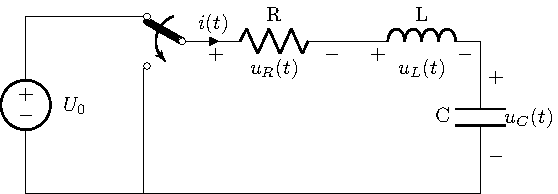
\includegraphics{../figs/transitorio_circuitoRLC_serie.pdf}
  \caption{Circuito RLC serie}
  \label{fig:transitorio_circuito_RLC_serie}
\end{figure}

Una vez el interruptor cambia de posición, se tiene el circuito de la
Figura~\ref{fig:transitorio_serie_t0+}, por la 2LK, se cumple que:
\[
  Ri(t) + L\diff{i(t)}{t} + \frac{1}{C}\int_{-\infty}^t i(t')
  \mathrm{d}t' = 0
\]

\[
  L\diff[2]{i}{t} + R\diff{i}{t} + \frac{1}{C} i = 0 \Rightarrow
  {\diff[2]{i}{t} + \frac{R}{L} \diff{i}{t} + \frac{1}{LC} i = 0}
\]
A partir del polinomio característico:
\[
  \lambda^2 + \frac{R}{L} \lambda + \frac{1}{LC} = 0 \Rightarrow
  \lambda_{1,2} = -\frac{R}{2L} \pm \sqrt{\left(\frac{R}{2L}\right)^2
    - \frac{1}{LC}}
\]
\begin{figure}[H]
  \centering
  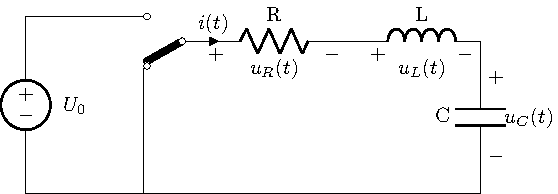
\includegraphics{../figs/transitorio_circuitoRLC_serie_t0+.pdf}
  \caption{Circuito RLC serie en $t>0$ (respuesta natural)}
  \label{fig:transitorio_serie_t0+}
\end{figure}

Haciendo los cambios de variable:
\begin{equation*} {\dfrac{R}{L}=2\,\xi\,\omega_n}\qquad \qquad
  {\dfrac{1}{LC}=\omega_n^2}
\end{equation*}
donde $\omega_n$ es la pulsación natural no amortiguada y $\xi$, el
factor de amortiguamiento, el polinomio característico queda:
\begin{equation*}
  \lambda^2+2\,\xi\,\omega_n\,\lambda + \omega_n^2=0 \Rightarrow \lambda_{1,2}=-\omega_n\left(\xi\pm\sqrt{\xi^2-1}\right)
\end{equation*}
En función del valor que tenga el factor de amortiguamiento $\xi$, las
raíces serán reales y distintas, una raíz real doble, o una raíz
compleja y su conjugada (con parte real o sin ella) teniendo el
circuito diferente comportamiento.
	
\begin{remark}
  Se pueden hacer también los siguientes cambios de variable:
  \begin{equation*} {\dfrac{R}{L}=2\,\alpha}\qquad \qquad
    {\dfrac{1}{LC}=\omega_n^2}
  \end{equation*}
  donde $\omega_n$ es la pulsación natural no amortiguada y $\alpha$,
  el coeficiente de amortiguamiento exponencial, quedando el polinomio
  característico:
  \begin{equation*}
    \lambda^2+2\,\alpha\,\lambda + \omega_n^2=0 \Rightarrow \lambda_{1,2}=-\alpha \pm \sqrt{\alpha^2 - \omega_0^2}
  \end{equation*}
  En este caso, es necesario conocer también el valor de $\omega_d$
  (pulsación natural amortiguada), que se obtiene a partir de:
  \begin{equation*}
    \omega_d=\sqrt{\omega_n^2-\alpha^2}
  \end{equation*}
\end{remark}
	
\begin{itemize}
\item \textbf{Sistema sobreamortiguado.} Cuando $\xi>1$ (o
  $\alpha>\omega_n$), el polinomio característico tiene \textbf{dos
    raíces reales distintas, negativas} ($\lambda_1\neq\lambda_2$). La
  respuesta natural es:
  \begin{equation*}
    i_n(t)=K_1\,\mathrm{e}^{\lambda_1\,t}+K_2\,\mathrm{e}^{\lambda_2\,t}   
  \end{equation*}
  con $K_1$ y $K_2$ constantes reales
  (Figura~\ref{fig:sobreamortiguado_HKD}).
  \begin{figure}[H]
    \centering 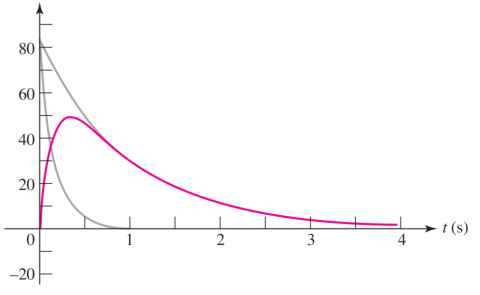
\includegraphics{../figs/Sobreamortiguado_HKD.pdf}
    \caption{Respuesta en un circuito sobreamortiguado}
    \label{fig:sobreamortiguado_HKD}
  \end{figure}
\item \textbf{Sistema críticamente amortiguado.} Cuando $\xi=1$ (o
  $\alpha=\omega_n$), el polinomio característico tiene \textbf{una
    raíz real doble} ($\lambda_1=\lambda_2=\lambda$). La respuesta
  natural es:
  \begin{equation*}
    i_n(t)=\mathrm{e}^{\lambda\,t}(K_1\,+K_2\,t)   
  \end{equation*}
  siendo $K_1$ y $K_2$ constantes
  reales(Figura~\ref{fig:criticamenteamortiguado_HKD}).
  \begin{figure}[H]
    \centering
    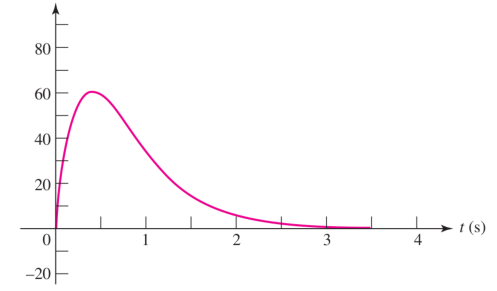
\includegraphics{../figs/AmortiguamientoCritico_HKD.pdf}
    \caption{Respuesta en un circuito críticamente amortiguado}
    \label{fig:criticamenteamortiguado_HKD}
  \end{figure}
\item \textbf{Sistema subamortiguado.} Cuando $0<\xi<1$ (o
  $\alpha<\omega_n$), el polinomio característico tiene \textbf{una
    raíz compleja y su conjugada} ($\lambda=a\pm b\,\mathrm{i}$). La
  respuesta natural es:
  \begin{equation*}
    i_n(t)=\mathrm{e}^{-\omega_n\,\xi \,t}\left[K_1\,\cos(\omega_n\,\sqrt{1-\xi^2}\,t)+K_2\,\sin(\omega_n\,\sqrt{1-\xi^2}\,t) \right]
  \end{equation*}
  o empleando $\alpha$ y $\omega_n$:
  \begin{equation*}
    i_n(t)=\mathrm{e}^{-\alpha \,t}\left[K_1\,\cos(\omega_d \,t)+K_2\,\sin(\omega_d\,t) \right]
  \end{equation*}
  siendo $K_1$ y $K_2$ constantes reales
  (Figura~\ref{fig:subamortiguado}).
  \begin{figure}[H]
    \centering
    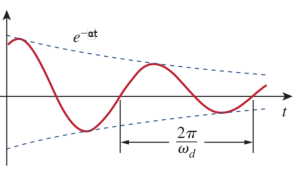
\includegraphics[width=0.45\linewidth]{../figs/Subamortiguado_AS.pdf}
    \caption{Respuesta en un circuito subamortiguado}
    \label{fig:subamortiguado}
  \end{figure}
\end{itemize}
	
Para determinar las constantes, son necesarias dos tipos de
condiciones iniciales:
\begin{align*}
  i_L(0^+) &= i_L(0^-)\\
  u_L(t) = L \cdot \diff{i_L(t)}{t}& \rightarrow   \diff{i_L(t)}{t}[t = 0^+] = \frac{1}{L} u_L(0^+)
\end{align*}

Para obtener valores de las derivadas en el origen, hay que resolver
el circuito en \(t = 0^+\) empleando las condiciones de
continuidad. Analizando el circuito de la
Figura~\ref{fig:transitorio_serie_t0+}, se observa que las derivadas
en $t=0^+$:
\[
  \diff{i_L(t)}{t}[t = 0^+] = \frac{1}{L} u_L(0^+)
\]
\begin{align*}
  u_L(0^+) &= -u_R(0^+) - u_c(0^+)\\
  u_R(0^+) &= R i_L(0^+)
\end{align*}
\[ {\diff{i_L(t)}{t}[t = 0^+] = - \frac{1}{L}\left(R i_L(0^+) +
      u_c(0^+)\right)}
\]
\begin{remark}
  Las condiciones iniciales deben evaluarse teniendo en cuenta la
  respuesta forzada (si existe).
  \begin{align*}
    i_L(0^+) &= i_n(0^+) + i_{\infty}(0^+)\\
    \diff{i_L}{t}[t = 0^+] &= \diff{i_n}{t}[t = 0^+] + \diff{i_{\infty}}{t}[t = 0^+]  
  \end{align*}
\end{remark}
Como en el caso de los circuitos de primer orden, la respuesta
completa es:
\begin{equation*}
  i(t)=i_n(t)+i_\infty(t)
\end{equation*}
siendo $i_\infty(t)$ la respuesta en régimen permanente (que, en el
caso concreto de este caso, no existe al no haber fuentes en $t>0$).

\subsection{Circuito RLC paralelo}

Sea el circuito RLC paralelo mostrado en la
Figura~\ref{fig:transitorio_circuito_RLC_paralelo}, donde se cumple
que en $t = 0$ el interruptor cambia de posición, dejando al circuito
sin alimentación externa.
\begin{figure}[H]
  \centering
  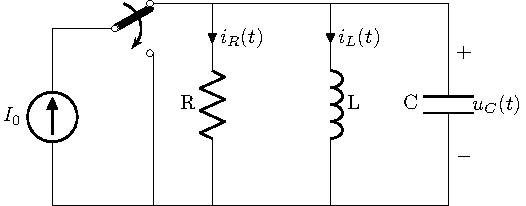
\includegraphics{../figs/transitorio_circuitoRLC_paralelo.pdf}
  \caption{Circuito RLC paralelo}
  \label{fig:transitorio_circuito_RLC_paralelo}
\end{figure}

Una vez el interruptor cambia de posición, se tiene el circuito de la
Figura~\ref{fig:transitorio_paralelo_t0+}, por la 1LK, se cumple que:
\[
  \dfrac{u(t)}{R} + C\diff{u(t)}{t} + \frac{1}{L}\int_{-\infty}^t
  u(t') \mathrm{d}t' = 0
\]

\[
  \diff[2]{u}{t} + \frac{1}{RC} \diff{u}{t} + \frac{1}{LC} u = 0
\]

A partir del polinomio característico:
\[
  \lambda^2 + \frac{1}{RC} \lambda + \frac{1}{LC} = 0
\]
\[
  \lambda_{1,2} = -\frac{1}{2RC} \pm
  \sqrt{\left(\frac{1}{2RC}\right)^2 - \frac{1}{LC}}
\]
\begin{figure}[H]
  \centering
  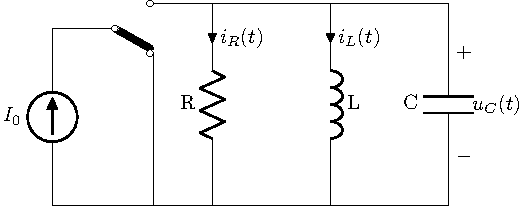
\includegraphics{../figs/transitorio_circuitoRLC_paralelo_t0+.pdf}
  \caption{Circuito RLC paralelo en $t>0$ (respuesta natural)}
  \label{fig:transitorio_paralelo_t0+}
\end{figure}

Haciendo los cambios de variable:
\begin{equation*} {\dfrac{1}{RC}=2\,\xi\,\omega_n}\qquad \qquad
  {\dfrac{1}{LC}=\omega_n^2}
\end{equation*}
donde $\omega_n$ es la pulsación natural no amortiguada y $\xi$, el
factor de amortiguamiento, el polinomio característico queda:
\begin{equation*}
  \lambda^2+2\,\xi\,\omega_n\,\lambda + \omega_n^2=0 \Rightarrow \lambda_{1,2}=-\omega_n\left(\xi\pm\sqrt{\xi^2-1}\right)
\end{equation*}
En función del valor que tenga el factor de amortiguamiento $\xi$, las
raíces serán reales y distintas, una raíz real doble y una raíz
compleja y su conjugada (con parte real o sin ella) teniendo el
circuito diferente comportamiento.
	
\begin{remark}
  Se pueden hacer también los siguientes cambios de variable:
  \begin{equation*} {\dfrac{1}{RC}=2\,\alpha}\qquad \qquad
    {\dfrac{1}{LC}=\omega_n^2}
  \end{equation*}
  donde $\omega_n$ es la pulsación natural no amortiguada y $\alpha$,
  el coeficiente de amortiguamiento exponencial, quedando el polinomio
  característico:
  \begin{equation*}
    \lambda^2+2\,\alpha\,\lambda + \omega_n^2=0 \Rightarrow \lambda_{1,2}=-\alpha \pm \sqrt{\alpha^2 - \omega_0^2}
  \end{equation*}
  En este caso, es necesario conocer también el valor de $\omega_d$
  (pulsación natural amortiguada), que se obtiene a partir de:
  \begin{equation*}
    \omega_d=\sqrt{\omega_n^2-\alpha^2}
  \end{equation*}
\end{remark}
	
\begin{itemize}
\item \textbf{Sistema sobreamortiguado.} Cuando $\xi>1$ (o
  $\alpha>\omega_n$), el polinomio característico tiene \textbf{dos
    raíces reales distintas, negativas} ($\lambda_1\neq\lambda_2$). La
  respuesta natural es:
  \begin{equation*}
    u_n(t)=K_1\,\mathrm{e}^{\lambda_1\,t}+K_2\,\mathrm{e}^{\lambda_2\,t}   
  \end{equation*}
  con $K_1$ y $K_2$ constantes reales.
\item \textbf{Sistema críticamente amortiguado.} Cuando $\xi=1$ (o
  $\alpha=\omega_n$), el polinomio característico tiene \textbf{una
    raíz real doble} ($\lambda_1=\lambda_2=\lambda$). La respuesta
  natural es:
  \begin{equation*}
    u_n(t)=\mathrm{e}^{\lambda\,t}(K_1\,+K_2\,t)   
  \end{equation*}
  siendo $K_1$ y $K_2$ constantes reales.
\item \textbf{Sistema subamortiguado.} Cuando $0<\xi<1$ (o
  $\alpha<\omega_n$), el polinomio característico tiene \textbf{una
    raíz compleja y su conjugada} ($\lambda=a\pm b\,\mathrm{i}$). La
  respuesta natural es:
  \begin{equation*}
    u_n(t)=\mathrm{e}^{-\omega_n\,\xi \,t}\left[K_1\,\cos(\omega_n\,\sqrt{1-\xi^2}\,t)+K_2\,\sin(\omega_n\,\sqrt{1-\xi^2}\,t) \right]
  \end{equation*}
  o empleando $\alpha$ y $\omega_n$:
  \begin{equation*}
    u_n(t)=\mathrm{e}^{-\alpha \,t}\left[K_1\,\cos(\omega_d \,t)+K_2\,\sin(\omega_d\,t) \right]
  \end{equation*}
  siendo $K_1$ y $K_2$ constantes reales.
\end{itemize}
	
Para determinar las constantes, son necesarias dos tipos de
condiciones iniciales:
\begin{align*}
  u_C(0^+) &= u_C(0^-)\\
  i_C(t) = C \cdot \diff{u_C(t)}{t}& \rightarrow   \diff{u_C(t)}{t}[t = 0^+] = \frac{1}{C} i_C(0^+)
\end{align*}

Para obtener valores de las derivadas en el origen, hay que resolver
el circuito en \(t = 0^+\) empleando las condiciones de
continuidad. Analizando el circuito de la
Figura~\ref{fig:transitorio_paralelo_t0+}, se observa que las
derivadas en $t=0^+$:
\[
  \diff{u_C(t)}{t}[t = 0^+] = \frac{1}{C} i_C(0^+)
\]
\begin{align*}
  i_C(0^+) &= -i_R(0^+) - i_L(0^+)\\
  i_R(0^+) &= \dfrac{1}{R} u_C(0^+)
\end{align*}
\[ {\diff{u_C(t)}{t}[t = 0^+] = - \frac{1}{C}\left(\frac{1}{R}
      u_C(0^+) + i_L(0^+)\right)}
\]
\begin{remark}
  Las condiciones iniciales deben evaluarse teniendo en cuenta la
  respuesta forzada (si existe).
  \begin{align*}
    i_L(0^+) &= i_n(0^+) + i_{\infty}(0^+)\\
    \diff{i_L}{t}[t = 0^+] &= \diff{i_n}{t}[t = 0^+] + \diff{i_{\infty}}{t}[t = 0^+]  
  \end{align*}
\end{remark}
Como en el caso de los circuitos de primer orden, la respuesta
completa es:
\begin{equation*}
  u(t)=u_n(t)+u_\infty(t)
\end{equation*}
siendo $u_\infty(t)$ la respuesta en régimen permanente (que, en el
caso concreto de este caso, no existe al no haber fuentes en $t>0$).
	
\subsection{Procedimiento general}
	
El \textbf{proceso general} de cálculo de transitorios en una red de
segundo orden sigue los siguientes pasos:
\begin{enumerate}
\item Dibujar el circuito para $t < 0$:
  \begin{itemize}
  \item Obtener los valores de $i_L(0^-)$ y $u_C(0^-)$
  \item Aplicar el principio de continuidad para determinar $i_L(0^+)$
    y $u_C(0^+)$ (según Sección~\ref{sec:condiciones_iniciales})
  \end{itemize}
\item Dibujar el circuito para \(t > 0\), caracterizando los elementos
  pasivos por su impedancia operacional
  (Sección~\ref{sec:operador_D}):
  \begin{itemize}
  \item Obtener la ecuación diferencial del sistema aplicando métodos
    de análisis generales
  \item Determinar la solución natural de la ecuación diferencial,
    especificando también el tipo de sistema. La ecuación homogénea
    del circuito ($g(t)=0$) es de la forma:
    \begin{equation*}
      a_2\,y''(t)+a_1\,y'(t)+a_0\,y(t)=0\Rightarrow {y''(t)+\dfrac{a_1}{a_2}\,y'(t)+\dfrac{a_0}{a_2}y(t)=0}
    \end{equation*}
    Haciendo los cambios de variable:
    \begin{equation}\label{eq:xi-omega_n}
      {\dfrac{a_1}{a_0}=2\,\xi\,\omega_n}\qquad \qquad
      {\dfrac{a_0}{a_2}=\omega_n^2}
    \end{equation}
    donde $\omega_n$ es la pulsación natural no amortiguada y $\xi$,
    el factor de amortiguamiento, el polinomio característico queda:
    \begin{equation*}
      \lambda^2+2\,\xi\,\omega_n\,\lambda + \omega_n^2=0 \Rightarrow \lambda_{1,2}=-\omega_n\left(\xi\pm\sqrt{\xi^2-1} \right)
    \end{equation*}
    En función del valor que tenga el coeficiente de amortiguamiento
    $\xi$, el sistema puede ser:
    \begin{itemize}
    \item \textit{Sistema sobreamortiguado.} Cuando $\xi>1$, el
      polinomio característico tiene {dos raíces reales distintas}
      ($\lambda_1\neq\lambda_2$), y se dice que el sistema es
      {sobreamortiguado}. La solución general (respuesta natural) es:
      \begin{equation*}
        y_g(t)=K_1\,\mathrm{e}^{\lambda_1\,t}+K_2\,\mathrm{e}^{\lambda_2\,t}   
      \end{equation*}
      En función de los valores que tome $K_1$ y $K_2$, que son
      constantes reales, la función que se tiene es creciente o
      decreciente. Estos sistemas suelen ser lentos, necesitando
      tiempos muy elevados para alcanzar el valor final. Además, la
      respuesta durante el transitorio no sobrepasa nunca el valor de
      régimen permanente.
    \item \textit{Sistema críticamente amortiguado.} Cuando $\xi=1$,
      el polinomio característico tiene {una raíz real doble}
      ($\lambda_1=\lambda_2=-\xi\,\omega_n=-\omega_n$), y se dice que
      el sistema es {críticamente amortiguado}. La solución general
      (respuesta natural) es:
      \begin{equation*}
        y_g(t)=\mathrm{e}^{-\omega_n\,t}(K_1\,+K_2\,t)   
      \end{equation*}
      siendo $K_1$ y $K_2$ constantes reales. En este caso, el tiempo
      hasta alcanzar el valor final es el menor posible, sin dar lugar
      a sobreoscilaciones.
    \item \textit{Sistema subamortiguado.} Cuando $0<\xi<1$, el
      polinomio característico tiene {una raíz compleja y su
        conjugada}
      ($\lambda=a\pm b\,\mathrm{i}=-\omega_n\,\xi\pm
      \omega_n\,\sqrt{1-\xi^2}\,\mathrm{i}$), y se dice que el sistema
      es {subamortiguado}. La solución general (respuesta natural) es:
      \begin{equation*}
        y_g(t)=\mathrm{e}^{-\omega_n\,\xi \,t}\left[K_1\,\cos(\omega_n\,\sqrt{1-\xi^2}\,t)+K_2\,\sin(\omega_n\,\sqrt{1-\xi^2}\,t) \right]  
      \end{equation*}
      que puede escribirse como:
      \begin{equation*}
        y_g(t)=M\,\mathrm{e}^{-\omega_n\,\xi \,t}\,\sin\left(\omega_n\,\sqrt{1-\xi^2}\,t + \theta \right)
      \end{equation*}
      donde $M=\sqrt{K_1^2+K_2^2}$ y $\tan(\theta)=\frac{K_2}{K_1}$,
      siendo $K_1$ y $K_2$ constantes reales.
    \end{itemize}
    % \subsubsection{Sistema no amortiguado (oscilante)}
    % Cuando $\xi=0$, el polinomio característico tiene \textbf{una
    % raíz compleja y su conjugada}, pero sin parte real
    % ($\lambda=\pm \omega_n\,\mathrm{i}$), y se dice que el sistema
    % es \textbf{no amortiguado} (u oscilante). La solución general
    % (respuesta natural), haciendo los mismos cambios que en la
    % Sección~\ref{sec:subamortiguado}, es:
    % \begin{equation*}
    % 	 y_g(t)=M\,\sin\left(\omega_n\,t + \theta \right)
    % \end{equation*}
  \item Calcular la respuesta en régimen permanente (solución
    particular, que corresponde a $t=\infty$), según el tipo de
    alimentación del circuito:
    \begin{itemize}
    \item \textit{Corriente continua}: sustituir las bobinas por
      cortocircuitos y los condensadores por circuitos abiertos
    \item \textit{Corriente alterna senoidal}: resolver el circuito
      por el método fasorial
    \item \textit{Otro tipo de forma de onda}: determinar la solución
      particular de la ecuación diferencial
    \end{itemize}
  \end{itemize}
\item Determinar las constantes de la ecuación:
  \begin{enumerate}
  \item Dibujar el circuito en el instante $t=0^+$, sustituyendo las
    bobinas y condensadores por fuentes de intensidad y tensión,
    respectivamente, de valor $i_L(0^+)$ y $u_C(0^+)$
  \item Con este nuevo circuito, puramente resistivo, cualquier
    variable se puede obtener por superposición $\rightarrow$ se
    obtiene la primera condición de contorno
  \item Derivar la expresión de la variable en estudio,
    particularizada para $t=0^+$ $\rightarrow$ se obtiene la segunda
    condición de contorno
  \item Resolver el sistema de ecuaciones obtenido
  \end{enumerate}
\item Escribir la solución completa para $t>0$
\end{enumerate}
	
\begin{example}\label{ex.2o_orden}
  \textbf{El circuito de la Figura~\ref{fig:ejemplo_2orden} lleva en
    la situación indicada un tiempo suficientemente grande, de forma
    que se encuentra en régimen permanente. En el instante $t=0$, se
    cierra el interruptor. Determinar la intensidad $i(t)$ para
    $t>0$. }
  \begin{figure}[H]
    \centering 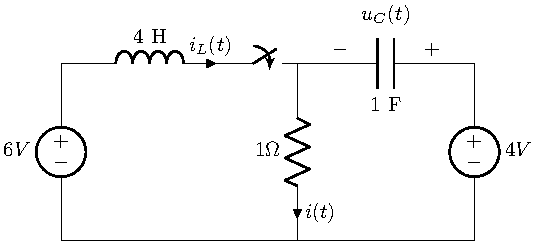
\includegraphics{../figs/ejemplo_2orden.pdf}
    \caption{Ejemplo~\ref{ex.2o_orden}}
    \label{fig:ejemplo_2orden}
  \end{figure}
	        
  \textbf{Cálculo de condiciones iniciales}
	        
  Antes de cerrar el interruptor, no circula corriente por la bobina,
  por lo que $i_L(0^-)=i_L(0^+)=0$ A, por continuidad.
	    
  El circuito de la derecha está en régimen permanente de corriente
  continua, por lo que el condensador se puede sustituir por un
  circuito abierto, no circulando así corriente por la resistencia. De
  este modo, $u_C(0^-)=u_C(0^+)=4$ V, por continuidad.
	    
	    
	    
  Una vez se cierra el interruptor, y caracterizando los elementos
  pasivos por su impedancia operacional, se tiene el circuito de la
  Figura~\ref{fig:ejemplo_2orden1}.
  \begin{figure}[H]
    \centering 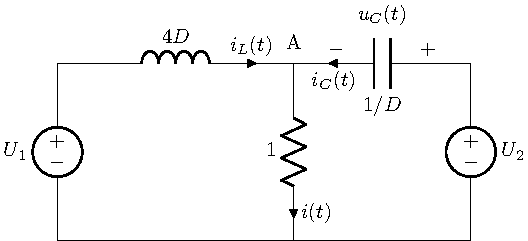
\includegraphics{../figs/ejemplo_2orden1.pdf}
    \caption{Circuito tras cerrar el interruptor}
    \label{fig:ejemplo_2orden1}
  \end{figure}
	    
  \textbf{Obtención de la ecuación diferencial}
	    
  Aplicando el método de nudos modificados, suponiendo que todas las
  corrientes salieran del nudo $A$, se tiene que:
  \begin{align*}
    0&=i_L(t)+i(t)+i_C(t)\\
    i_L(t)&=\dfrac{U_A-0-U_1}{4\,D}=\dfrac{U_A-U_1}{4\,D}\\
    i(t)&=\dfrac{U_A-0}{1}=U_A\\
    i_C(t)&=\dfrac{U_A-0-U_2}{\frac{1}{D}}=D\,U_A-D\,U_2\\
  \end{align*}
  Sustituyendo en la 1LK y operando, se obtiene que:
  \begin{equation*}
    U_A=\dfrac{U_1+4\,D^2\,U_2}{4\,D^2+4\,D+1}
  \end{equation*}
  Por tanto, dado que $i(t)=\frac{U_A}{1}$, se llega a la conclusión
  de que:
  \begin{equation*}
    i(t)=\dfrac{U_1+4\,D^2\,U_2}{4\,D^2+4\,D+1}\Rightarrow \left(4\,D^2+4\,D+1\right) i(t)=U_1+4\,\cancelto{0}{D^2\,U_2}\Rightarrow \left(4\,D^2+4\,D+1\right) i(t)=6
  \end{equation*}
  que es la ecuación diferencial a resolver.
	    
  \textbf{Determinar la solución natural}
	    
  La ecuación homogénea es:
  \begin{equation*}
    \left(4\,D^2+4\,D+1\right) i(t)=4\diff[2]{i(t)}{t}+4\diff{i(t)}{t}+1=0
  \end{equation*}
  y considerando las expresiones de~\eqref{eq:xi-omega_n}:
  \begin{align*}
    \dfrac{1}{4}&=\omega_n^2\Rightarrow \omega_n=\dfrac{1}{2}\\
    1&=2\,\xi\,\omega_n=2\,\xi\,\dfrac{1}{2}\Rightarrow \xi = 1
  \end{align*}
  por lo que se trata de un sistema críticamente
  amortiguado. Resolviendo el polinomio característico, se tiene que:
  \begin{equation*}
    \lambda_1=\lambda_2=\lambda=-\dfrac{1}{2}
  \end{equation*}
  por lo que:
  \begin{equation*}
    i_g(t)=\mathrm{e}^{-\frac{1}{2}\,t}(K_1\,+K_2\,t) 
  \end{equation*}
	    
  \textbf{Determinar la solución en régimen permanente}
	    
  Al tratarse de un circuito de corriente continua, el régimen
  permanente la bobina se comporta como un cortocircuito y el
  condensador como un circuito abierto, quedando la fuente de 4 V
  aislada y recibiendo la resistencia una tensión de 6 V. Por la ley
  de Ohm:
  \begin{equation*}
    i_\infty(t)=\dfrac{U_R}{R}=\dfrac{6}{1}=6\,\text{A}
  \end{equation*}
	    
  \textbf{Determinar las constantes}
	    
  Se sustituye la bobina por una fuente de intensidad de valor 0 A y
  el condensador por una fuente de tensión de 4 V, como en la
  Figura~\ref{fig:ejemplo_2orden1}.
  \begin{figure}[H]
    \centering
    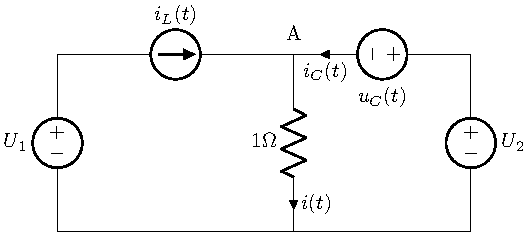
\includegraphics[width=0.45\linewidth]{../figs/ejemplo_2orden2.pdf}
    \caption{Determinar las constantes de integración}
    \label{fig:ejemplo_2orden2}
  \end{figure}
	    
  Por tanto, la corriente en la resistencia queda determinada por las
  dos fuentes de tensión ubicadas a su derecha:
  \begin{equation*}
    u_R(t)=U_2-u_C(t)\Rightarrow i(t)=\dfrac{u_R(t)}{R}
  \end{equation*}
  cuya derivada es:
  \begin{equation*}
    \diff{i(t)}{t}=\dfrac{\cancelto{0}{\diff{U_2}{t}}-\diff{u_C(t)}{t}}{R}=-\dfrac{1}{R}\,\diff{u_C(t)}{t}=-\dfrac{i_C(t)}{R\,C}
  \end{equation*}
  La intensidad del condensador, por la 1LK:
  \begin{equation*}
    i_C(t)=i(t)-i_L(t)
  \end{equation*}
  Dando ahora los valores de las condiciones iniciales a bobina y
  condensador, y particularizando para $t=0^+$, se obtienen las
  constantes $K_1$ y $K_2$:
  \begin{align*}
    i(0^+)&=\dfrac{4-4}{1}=0\\
    \diff{i}{t}[t = 0^+]&=-\dfrac{i(0^+)-i_L(0^+)}{R\,C}=-\dfrac{0-0}{1\cdot 1}=0
  \end{align*}
  Imponiendo estas condiciones a la solución de la ecuación
  diferencial:
  \begin{equation*}
    i(t)=6+\mathrm{e}^{-\frac{1}{2}\,t}(K_1\,+K_2\,t)\Rightarrow
    \begin{cases}
      i(0^+)=0=6+\mathrm{e}^{-\frac{1}{2}\,0}(K_1\,+K_2\,0)=6+K_1\Rightarrow K_1=-6\\
      \diff{i}{t}[t = 0^+]=0=\mathrm{e}^{-\frac{1}{2}0}\left[-\frac{1}{2}(K_1+K_2\cdot 0)+K_2 \right]\Rightarrow K_2=-3
    \end{cases}
  \end{equation*}
  por lo que la corriente para $t>0$ es:
  \begin{equation*}
    i(t)=6+\mathrm{e}^{-\frac{1}{2}\,t}(-6-3\,t)
  \end{equation*}
	    
\end{example}
	
%%% Local Variables:
%%% mode: latex
%%% TeX-master: "TC"
%%% ispell-local-dictionary: "castellano"
%%% End:
